\providecommand{\main}{..}
\documentclass[\main/main.tex]{subfiles}
\begin{document}
\chapter{Algoritmi di approssimazione}
\begin{multicols}{2}
\begin{definition}[Algoritmo approssimato]
    Un algoritmo \(\rho\)-approssimato risolve istanze arbitrarie di un problema NP in tempo polinomiale identificando una soluzione che è al più a un fattore \(\rho\) dalla soluzione ottima. Il problema principale con questa categoria di algoritmi sta nel dimostrare che la soluzione prodotta è \textbf{vicina} all'ottimo, senza però conoscere quale sia il valore ottimo.
\end{definition}
\section{Load balancing problem}
\begin{problem}[Load balancing]
    Dato un insieme di \(m\) macchine \(M_1, \ldots, M_m\) ed un insieme di \(n\) lavori con associato un tempo di elaborazione \(t_j\). L'obbiettivo è assegnare ogni lavoro a una macchina in modo tale che il tempo di esecuzione sia il più bilanciato il possibile: vogliamo minimizzare il tempo di esecuzione assegnato a una macchina massimo (\textbf{makespan}).
\end{problem}
\begin{example}[Greedy Balance]
    Un possibile algoritmo molto semplice per approcciare l'LBP è un algoritmo che itera lungo la lista dei lavori e assegna il lavoro \(j\)-esimo alla macchina il cui carico è minore sino ad ora.
\end{example}
\begin{analysis}[Lowerbound per Greedy Balance]
    Sia \(T\) il \textbf{makespan} dell'assegnamento ottenuto dall'algoritmo. Vogliamo mostrare che \(T\) non è troppo maggiore del makespan ottimo \(T^*\). Per fare questo confronto però dobbiamo identificare il valore \(T^*\), che non possiamo calcolare. Ne cerchiamo pertanto un \textbf{minorante}, e un buon candidato è il \textbf{makespan medio}, dato che almeno una delle \(m\) macchine dovrà svolgere una frazione \(\sfrac{1}{m}\) del lavoro.
    \[
        T^{*} \geq \frac{1}{m} \sum_{j} t_{j}
    \]
    In alcuni casi esistono però tempi legati a lavori che sono maggiori della media, e pertanto il minorante identificato precedentemente risulterebbe non sufficientemente forte. Si va ad aggiungere quindi un ulteriore minorante: \(
        T^{*} \geq \max _{j} t_{j}
    \)
\end{analysis}
\begin{lemma}[Approssimazione del Greedy Balance]
    L'algoritmo Greedy Balance produce un assegnamento dei lavori alle macchine con makespan \(T \leq 2 T^{*}\).
\end{lemma}
\begin{proof}[Approssimazione del Greedy Balance]
    Consideriamo una macchina \(M_i\) cui viene assegnato il carico massimo \(T\). Quale è stato l'ultimo lavoro \(j\) assegnato a \(M_i\)? Se \(t_j\) non è eccessivamente più grande degli altri lavori, potremmo usare il minimale ottenuto tramite la media, altrimenti quello ottenuto tramite il massimo. 
    
    Quando assegniamo il lavoro \(j\) alla macchina \(M_i\), la macchina \(M_i\) ha il carico minore di tutte le altre macchine ed era pari a \(T_i - t_j\). Ne segue che:
    \[
        T_{i}-t_{j} \leq \frac{1}{m} \sum_{k} T_{k}
    \]
    Ma il valore \(\sum_{k} T_{k} = \sum_{j} t_{j}\), per cui il valore a destra coincide con il lower bound della media:
    \[
        T_{i}-t_{j} \leq T^{*}
    \]
    Considerando ora il lower bound del massimo, che dice che \(t_j \leq T^*\):
    \[
        T_{i}=\left(T_{i}-t_{j}\right)+t_{j} \leq 2 T^{*}
    \]
    Da cui la tesi.
\end{proof}
\begin{example}[Greedy Sorted Balance]
    Si tratta di un algoritmo migliore del Greedy Balance, che procede quasi come il precedente ma i lavori sono assegnati utilizzando una lista ordinata in ordine decrescente.
\end{example}
\begin{analysis}[Identificare un lowerbound per Greedy Sorted Balance]
    Avendo \(m\) macchine, se esistono meno di \(m\) lavori la soluzione identificata dall'algoritmo sarà banalmente ottima, se invece abbiamo più di \(m\) lavori possiamo introdurre un altro valore minimale.
    
    Consideriamo i primi \(m+1\) lavori ordinati: ognuno richiede almeno tempo \(t_{m+1}\). Siccome esistono \(m+1\) lavori e solo \(m\) macchine, ci deve essere una macchina cui viene assegnato due lavori, e questa macchina avrà tempo di calcolo \(2t_{m+1}\).
\end{analysis}
\begin{lemma}[Approssimazione del Greedy Sorted Balance]
    L'algoritmo Greedy Sorted Balance produce un assegnamento dei lavori alle macchine con makespan \(T \leq \frac{3}{2} T^{*}\).
\end{lemma}
\end{multicols}
\begin{proof}[Approssimazione del Greedy Sorted Balance]
    Consideriamo la macchina \(M_i\) con carico massimo. Se ad essa è stato assegnato un solo lavoro allora la soluzione è ottimale, altrimenti la macchina ha almeno due lavori.
    
    Sia \(t_j\) l'ultimo lavoro assegnato alla macchina. Il lavoro deve essere \(j \geq m+1\) dato che i primi \(m\) lavori sono stati assegnati ad \(m\) macchine distinte. Di conseguenza, \(t_j \leq t_{m+1} \leq \frac{1}{2} T^*\). In precedenza usando i minimali avevamo ottenuto le disuguaglianze \(T_{i}-t_{j} \leq T^{*}\) e \(t_{j} \leq T^{*}\), ma in questo caso la seconda disuguaglianza può essere resa più stringente: \(t_{j} \leq \frac{1}{2} T^{*}\).
    
    Sommando le due disuguaglianze otteniamo:
    \[
        T_{i} \leq \frac{3}{2} T^{*}
    \]
\end{proof}
\section{Set Cover}
\begin{problem}[Set Cover]
    Considerando un insieme di \(n\) elementi \(U\) ed una lista \(S_1, S_2, \ldots, S_m\) di sottoinsiemi di \(U\). Una \textbf{set cover} è una collezione di insiemi la cui unione è uguale a \(U\). Nella versione pesata, ad ogni insieme \(S_1, S_2, \ldots, S_m\) è assegnato un peso \(w_i \geq 0\), ed il nostro scopo è identificare una \textbf{set cover} di peso minimo.
\end{problem}
\begin{definition}[Algoritmo greedy per il Set Cover]
    L'algoritmo greedy costruisce la \textbf{set cover} un insieme per volta, scegliendo ad ogni iterazione l'insieme di peso minimo che copre più elementi. Se chiamiamo \(R\) l'insieme parziale di elementi ancora non coperti, definiamo il peso assegnato ad ogni insieme come:
    \[
        \frac{w_i}{S_i \cap R}
    \]
    Ogni volta che viene aggiunto un set \(S_i\) andiamo a rimuoverne gli elementi da \(R\) e l'algoritmo termina la sua iterazione quando \(R\) risulta vuoto.
\end{definition}
\section{Il problema dello zaino}
\begin{problem}[Il problema dello zaino]
    Si vogliono mettere \(n\) oggetti in uno zaino di capacità finita \(W\), ogni oggetto ha un peso \(w_i\) ed un valore \(v_i\): vogliamo massimizzare il valore totale degli oggetti trasportati senza superare la capacità massima.
\end{problem}
\begin{definition}[Approssimazione polinomiale del problema dello zaino]
    Dopo aver scelto un parametro di arrotondamento \(b\), il cui valore fissiamo in base al valore dell'approssimazione \(1+\epsilon\) che vogliamo raggiungere:
    \[
        b = \frac{\epsilon}{2n}\max_i v_i
    \]
    Calcoliamo i pesi arrotondati:
    \[
        \tilde{v}_i = \ceil{\frac{v_i}{b}}\cdot b
    \]
    Procediamo quindi a risolvere il problema dello zaino con i pesi arrotondati. Il problema dello zaino con i valori \(\tilde{v}_i\) hanno lo stesso insiemi di soluzioni ottime, i valori ottimi differiscono di un fattore \(b\) e i valori scalati sono interi.
\end{definition}
\clearpage
\section{Center selection problem}
\begin{multicols}{2}
\begin{problem}[Center selection problem]
    Dato un insieme \(S\) composto da \(n\) punti (i luoghi), vogliamo scegliere un insieme \(C\) di \(k\) punti che risultino \textbf{centrali} rispetto ai punti di \(S\). Diciamo che l'insieme \(C\) forma una \(r\)-cover se ogni punto si \(S\) si trova a una distanza al più pari a \(r\) da uno dei centri. Il valore minimo di \(r\) per cui \(C\) è una \(r\)-cover viene chiamato \textbf{raggio di copertura} di \(C\): l'obbiettivo è selezionare i \(k\) punti di \(C\) in modo tale da minimizzare \(r\).
\end{problem}
\begin{definition}[Approccio Greedy semplice per center selection problem]
    Un algoritmo Greedy molto semplice procederebbe scegliendo come primo punto il migliore possibile se dovesse scegliere un solo centro, quindi procederebbe ad aggiungere centri in modo da ridurre ad ogni step il massimo possibile il \textbf{raggio di copertura}.
\end{definition}
\begin{observation}[Limiti di un approccio Greedy semplice]
    Prendiamo in considerazione un'istanza con due luoghi in \(S\) e \(k=2\). Sia \(d\) la distanza tra \(s\) e \(z\): un algoritmo greedy semplice inizierebbe scegliendo il punto a metà tra i due ed il raggio di copertura sarebbe \(\frac{d}{2}\). Ma ora qualsiasi altra posizione venga scelta per il secondo centro, uno dei due punti di \(S\) lo avrebbe più vicino e il \textbf{raggio di copertura non migliorerebbe}. Chiaramente per un'istanza di questo tipo la soluzione ottima sarebbe selezione i due punti stessi come centri, raggiungendo \textbf{raggio di copertura zero}.
\end{observation}
\begin{observation}[In che modo conoscere il raggio ottimo aiuta?]
    Supponiamo di conoscere il raggio ottimo \(r^*\) di una soluzione \(C^*\) e di dover individuare un insieme di centri \(C\) che non abbia un raggio troppo maggiore di \(r\): Consideriamo un qualsiasi luogo \(s \in S\). Deve esistere un centro \(c^* \in C^*\) che copre \(s\). Andremmo quindi a scegliere questo luogo \(s\) come centro per la nostra soluzione, non sapendo quale sia \(c^*\), e per coprire tutti i luoghi che \(c^*\) copre nella soluzione sconosciuta \(C^*\) andremmo a raddoppiare il raggio da \(r^*\) a \(2r^*\) (per diseguaglianza triangolare).
    
    Ogni insieme di centri \(C\) identificati da questo algoritmo ha raggio di copertura \(r \leq 2r^*\).
\end{observation}
\vfill\null
\columnbreak
\begin{lemma}[Esistenza di soluzione ottima con raggio \(r^*\)]
    Se l'algoritmo greedy che conosce il raggio ottimo \(r^*\) seleziona più di \(k\) centri, allora per ogni soluzione \(C^*\) di dimensione al più \(k\), il raggio di copertura è \(r\rnd{C^*} > r^*\).
\end{lemma}
\begin{proof}[Esistenza di soluzione ottima con raggio \(r^*\)]
    Ragioniamo per assurdo che esista una soluzione \(C^*\) di al più \(k\) centri con raggio di copertura \(r\rnd{C^*} \leq r^*\). Ogni centro \(c \in C\) selezionato dall'algoritmo è uno dei luoghi \(s \in S\), e l'insieme \(C^*\) ha raggio di copertura al più pari a \(r^*\), per cui deve esistere un centro \(c^* \in C^*\) che è al più a distanza \(r\) da un centro \(c \in C\).
    
    Vogliamo dimostrare che non esiste un centro \(c^* \in C^*\) che risulti vicino a due centri della soluzione \(C\): questo implicherebbe che ogni centro \(c \in C\) è vicino a un centro ottimo \(c^*\), ed ognuno di questi deve essere distinto e pertanto \(\abs{C^*} \geq \abs{C}\) e siccome \(\abs{C} > k\) si contraddirebbe l'assunzione che \(C^*\) contiene al più \(k\) centri.
    
    Procediamo quindi a mostrare che nessun centro ottimo \(c^* \in C^*\) può essere vicino a due centri \(c, c' \in C\). Ogni coppia di centri  \(c, c' \in C\) è separata da un distanza maggiore di \(2r^*\) per costruzione e quindi se il punto \(c^*\) fosse a distanza al più \(r^*\) da ognuno dovrebbe violare la disuguaglianza triangolare.
\end{proof}
\begin{observation}[Come procediamo senza conoscere il raggio ottimo?]
    Possiamo iniziare da un valore scelto arbitrariamente per \(r\), che sappiamo essere tra \(0\) e la distanza massima tra due luoghi qualsiasi \(r_{\text{max}}\). Un possibile valore è \(r=\frac{r_{\text{max}}}{2}\). In base all'algoritmo o possiamo identificare una soluzione di \(k\) centri con raggio di copertura al più pari a \(2r\) o possiamo concludere che non esiste una soluzione con raggio di copertura al più \(r\). Nel primo caso possiamo iterare ed abbassare la nostra approssimazione per \(r^*\), mentre nel secondo caso la dovremo aumentare.
    
    Si procede quindi ad iterare dicoticamente per identificare una stima sempre migliore del raggio di copertura, procedendo fino a che la distanza tra il raggio ottimo approssimato a uno step non cambia troppo dall'iterazione precedente.
    
    La soluzione ottenuta quindi risulta essere una \(2\)-approssimazione della soluzione ottima.
\end{observation}
\vfill\null
\begin{definition}[Algoritmo greedy per il problema della selezione dei centri]
    Procedendo in un modo simile all'algoritmo proposto, ma senza iterare sui possibili valori ottimali, dopo aver scelto come centro iniziare un punto \(s\) a caso, possiamo scegliere il luogo \(s\) più distante dal centro selezionato precedentemente. Se esiste un luogo a distanza \(2r\) da tutti gli altri centri scelti allora il punto \(s\) più distante deve essere parte dei centri.
\end{definition}
\begin{lemma}[Approssimazione dell'algoritmo greedy per il problema della selezione dei centri]
    L'algoritmo greedy identifica un insieme di \(k\) punti \(C\) tale che \(r\rnd{C} \leq 2r\rnd{C^*}\), dove \(C^*\) è un insieme ottimale di \(k\) punti.
\end{lemma}
\begin{proof}[Approssimazione dell'algoritmo greedy per il problema della selezione dei centri]
    Sia \(r^*\) il raggio di copertura minimo per un insieme di \(k\) centri. Procediamo assumendo per assurdo di dover identificare un insieme di \(k\) centri \(C\) con \(r\rnd{C} > 2r^*\). Sia \(s\) un luogo che è a distanza maggiore di \(2r^*\) da un qualsiasi centro in \(C\). Consideriamo qualche iterazione intermedia dell'algoritmo, in cui son stati selezionati alcuni centri in \(C'\). Supponiamo di procedere ad aggiungere \(c'\) in questa iterazione: riteniamo che \(c'\) è distante almeno \(2r^*\) da qualsiasi centro in \(C'\), dato che il luogo \(s\) è distante più di \(2r\) da tutti i centri del set \(C\), e quindi selezioniamo il luogo \(c\) che è il più distante da tutti gli altri centri scelti.
    
    Ne segue che l'algoritmo greedy è una implementazione corretta per le prime \(k\) iterazioni dell'algoritmo proposto precedentemente che conosceva il raggio ottimale \(r^*\): ad ogni iterazione aggiungiamo il punto a distanza maggiore di \(2r^*\) da ogni centro selezionato precedentemente.
    
    Ma l'algoritmo precedente avrebbe \(S' \neq \emptyset\) dopo aver selezionato \(k\) centri dato che \(s \in S'\), e quindi procederebbe a scegliere più di \(k\) centri concludendo alla fine che \(k\) centri non possono avere raggio di copertura \(r^*\). Questo contraddice la nostra scelta di \(r\), e la contraddizione prova che \(r\rnd{C} \leq 2r^*\).
\end{proof}
\begin{problem}[Problema dell'insieme dominante]
    Un \textbf{insieme dominante} per un grafo \(G = (V, E)\) è un sottoinsieme \(D\) di \(V\) tale che ogni vertice non in \(D\) è adiacente ad almeno un membro di \(D\). Il \textbf{numero di dominazione} è il numero di vertici nel più piccolo \textbf{insieme dominante} di \(G\).
    
    Il \textbf{problema dell'insieme dominante} consiste nel determinare se per un dato grafo è possibile trovare un insieme dominante di cardinalità inferiore a un dato \(k\). Si tratta di un problema NP-completo.
\end{problem}
\begin{theorem}[Inapprossimibilità del Center Selection problem]
    A meno che \textbf{P = NP}, non esiste nessuna \(\rho\)-approssimazione per il problema di Center Selection con \(\rho<2\).
\end{theorem}
\begin{proof}[Inapprossimibilità del Center Selection problem]
    Procediamo per assurdo assumendo che sia possibile realizzare un algoritmo con \(\rnd{2-\epsilon}\)-approssimazione per \textbf{center selection}: un tale algoritmo potrebbe essere utilizzato per risolvere il \textbf{problema dell'insieme dominante} (un noto problema NP-Completo) in tempo polinomiale.
    
    Sia \(G=\rnd{V, E}\) e \(k\in\N\) un'istanza di \textbf{problema dell'insieme dominante}. Costruiamo un'istanza \(G'\) di \textbf{center selection} i cui siti sono i vertici del grafo e le distanze sono definite come:
    \begin{align*}
        \begin{aligned}
            \operatorname{dist}(u, v) &=1 \text { se }(u, v) \in E \\
            \operatorname{dist}(u, v) &=2 \text { se }(u, v) \notin E
        \end{aligned}
    \end{align*}
    Il grafo \(G\) ha un \textbf{insieme dominante} di dimensione \(k\) se e solo se esistono \(k\) centri \(C^*\) con \(r\rnd{C^*} = 1\). Di conseguenza, se \(G\) ha un insieme dominante di dimensione \(k\), una algoritmo di \(2-\epsilon\)-approssimazione per \textbf{center selection} potrebbe trovare una soluzione \(C^*\) con \(r\rnd{C^*} = 1\), dato che non può usare nessun arco di distanza 2.
\end{proof}
\end{multicols}
\clearpage
\section{Il metodo del Pricing: Vertex Cover}
\begin{multicols}{2}
\begin{problem}[Vertex Cover]
    Un \textbf{vertex cover} in un grafo \(G = \rnd{V, E}\) è un insieme \(S \subseteq V\) tale che ogni lato abbia almeno un termine in \(S\). Nella versione pesata ad ogni vertice \(i \in V\) viene assegnato un peso \(w_i \geq 0\), e vorremmo trovare il \textbf{vertex cover} a peso minimo.
\end{problem}
\begin{lemma}[Approssimare Vertex Cover con Set Cover]
    È possibile utilizzare l'algoritmo di approssimazione del \textbf{Set Cover} per raggiungere un algoritmo con \(H\rnd{d}\)-approssimazione per la versione pesata del \textbf{Vertex Cover}, dove \(d\) è il grado massimo del grafo.
\end{lemma}
\begin{proof}[Approssimare Vertex Cover con Set Cover]
    Consideriamo un'istanza di \textbf{Vertex Cover pesato}, specificata da un grafo \(G = \rnd{V, E}\). Definiamo un'istanza di \textbf{Set Cover} con insieme \(U\) pari a \(E\) e per ogni nodo \(i\) definiamo il set \(S_i\) consistente di tutti i lati incidenti a un nodo \(i\) e diamo a questo insieme peso \(w_i\). Le \textbf{set cover} che coprono \(U\) corrispondono quindi precisamente a \textbf{vertex cover}. La massima dimensione degli insiemi \(S_i\) così definito coincide con il grado massimo \(d\).
    
    Ne segue che è possibile utilizzare l'algoritmo di approssimazione per Set Cover per trovare una soluzione al problema del \textbf{vertex cover pesato} il cui peso è una \(H\rnd{d}\)-approssimazione.
\end{proof}
\begin{observation}[Quanto è buona l'approssimazione del Vertex Cover col Set Cover?]
    L'approssimazione è piuttosto buona quando \(d\) è piccolo, ma peggiora mano a mano che \(d\) diventa più grande, arrivando a un limite logaritmico nel numero dei vertici.
\end{observation}
\vfill\null
\columnbreak
\begin{lemma}[Minimale del costo totale del pricing per Vertex Cover]
    Per qualsiasi vertex cover \(S^*\), e ogni insieme di prezzi non negativi \(p_e\), si ha che:
    \[
        \sum_{e \in E} p_e \leq w\rnd{S^*}
    \]
\end{lemma}
\begin{proof}[Minimale del costo totale del pricing per Vertex Cover]
    Consideriamo una vertex cover \(S^*\): per definizione di \textbf{equità del costo}, abbiamo che:
    \[
        \sum_{e = \rnd{i,j}} p_e \leq w_i \quad \forall i \in S^*
    \]
    Aggiungendo queste disuguaglianze su tutti i nodi in \(S^*\) otteniamo:
    \[
        \sum_{i \in S^{*}} \sum_{e=(i, j)} p_{e} \leq \sum_{i \in S^{*}} w_{i}=w\left(S^{*}\right)
    \]
    L'espressione sulla sinistra è una somma dei costi dei lati. Siccome \(S^*\) è una vertex cover, ogni lato \(e\) contribuisce al più un termine \(p_e\) al lato sinistro. Potrebbe infatti contribuire più di una copia di \(p_e\) alla somma, siccome potrebbe essere coperto da ambo i lati in \(S^*\). Ma i prezzi sono non-negativi, per cui la somma dei termini a sinistra è grande almeno quanto la somma di tutti i prezzi \(p_e\):
    \[
        \sum_{e \in E} p_{e} \leq \sum_{i \in S^{*}} \sum_{e=(i, j)} p_{e}
    \]
    Combinando questa disuguaglianza con quella ottenuta precedentemente otteniamo:
    \[
        \sum_{e \in E} p_{e} \leq w\left(S^{*}\right)
    \]
\end{proof}
\begin{definition}[Algoritmo greedy per Vertex Cover]
    Diciamo che un nodo \(i\) è \textbf{pagato} se risulta che \(\sum_{e=(i, j)} p_{e}=w_{i}\). Inizializziamo tutti i pesi \(p_e\) a zero, quindi iteriamo fintanto che esiste un lato di cui nessuno dei due vertici sono \textbf{pagati}: selezioniamo questo lato ed aumentiamo il prezzo \(p_e\) senza violare l'\textbf{equità del costo}. Quando il ciclo termina, la nostra vertex cover sarà l'insieme dei vertici \textbf{pagati}. 
\end{definition}
\clearpage
\begin{lemma}[Equità dell'algoritmo greedy per Vertex Cover]
    La \textbf{vertex cover} ed i prezzi \(P\) individuati dall'algoritmo greedy per Vertex Cover soddisfano l'uguaglianza:
    \[
        w(S) \leq 2 \sum_{e \in E} p_{e}
    \]
\end{lemma}
\begin{proof}[Equità dell'algoritmo greedy per Vertex Cover]
    Dato che tutti i nodi in \(S\) sono \textbf{pagati}, si ha che \(\sum_{e=(i, j)} p_{e}=w_{i} \quad \forall i \in S\). Sommando tutti i nodi in \(S\) otteniamo:
    \[
        w(S)=\sum_{i \in S} w_{i}=\sum_{i \in S} \sum_{e=(i, j)} p_{e}
    \]
    Un lato \(e = \rnd{i,j}\) può essere incluso nella somma del lato destro al più due volte (nel caso in cui sia \(i\) che \(j\) risultano nella \textbf{vertex cover} \(S\)), per cui si ottiene:
    \[
        w(S)=\sum_{i \in S} \sum_{e=(i, j)} p_{e} \leq 2 \sum_{e \in E} p_{e}
    \]
\end{proof}
\begin{lemma}[Algoritmo greedy per Vertex Cover è 2-approssimato]
    L'insieme \(S\) ritornato dall'algoritmo greedy per Vertex Cover è una \textbf{vertex cover} ed il suo costo è al più due volte il costo ottimo.
\end{lemma}
\begin{proof}[Algoritmo greedy per Vertex Cover è 2-approssimato]
    Se \(S\) per assurdo non fosse una \textbf{vertex cover} non andrebbe a coprire almeno un lato \(e = \rnd{i,j}\). Questo implicherebbe che ne \(i\) ne \(j\) sarebbero \textbf{pagati} ma questo impedirebbe all'algoritmo di uscire dal ciclo iterativo.
    
    Sia \(p\) l'insieme dei prezzi per l'algoritmo e sia \(S^*\) la vertex cover ottima. Siccome i prezzi sono \textbf{equi} vale che \(2 \sum_{e \in E} p_{e} \geq w(S)\) e siccome \(S\) è una \textbf{vertex cover} a prezzi non negativi vale che \(\sum_{e \in E} p_{e} \leq w\left(S^{*}\right)\). Ne segue che:
    \[
        w(S) \leq 2 \sum_{e \in E} p_{e} \leq 2 w\left(S^{*}\right)
    \]
\end{proof}
\end{multicols}
\begin{figure}
    \begin{subfigure}{0.49\textwidth}
        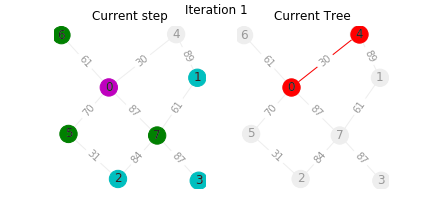
\includegraphics[width=\textwidth]{pricing/1.png}
    \end{subfigure}
    \begin{subfigure}{0.49\textwidth}
        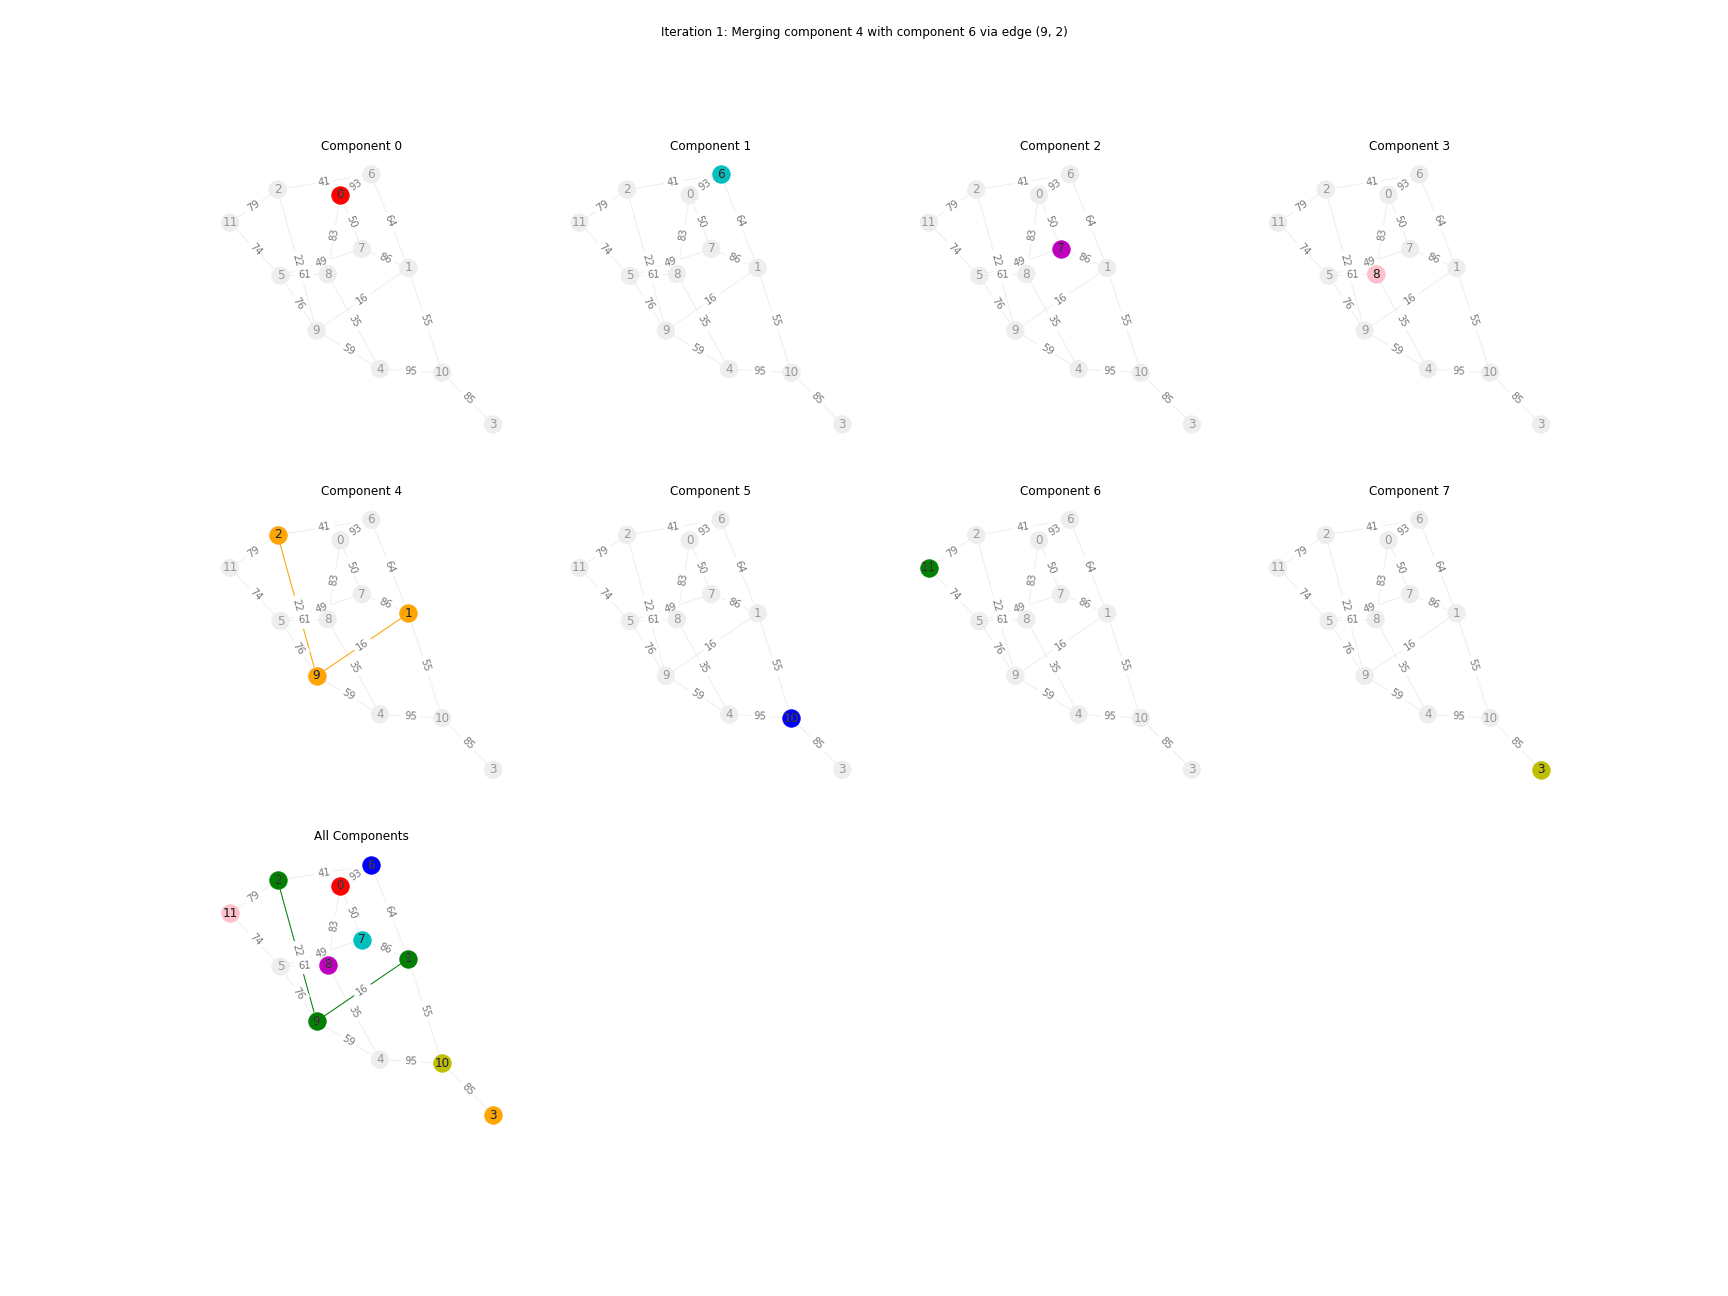
\includegraphics[width=\textwidth]{pricing/2.png}
    \end{subfigure}
    \begin{subfigure}{0.49\textwidth}
        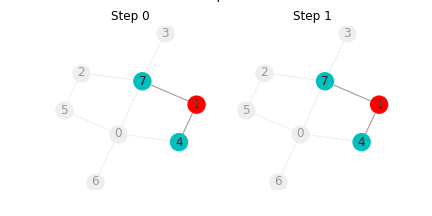
\includegraphics[width=\textwidth]{pricing/3.png}
    \end{subfigure}
    \begin{subfigure}{0.49\textwidth}
        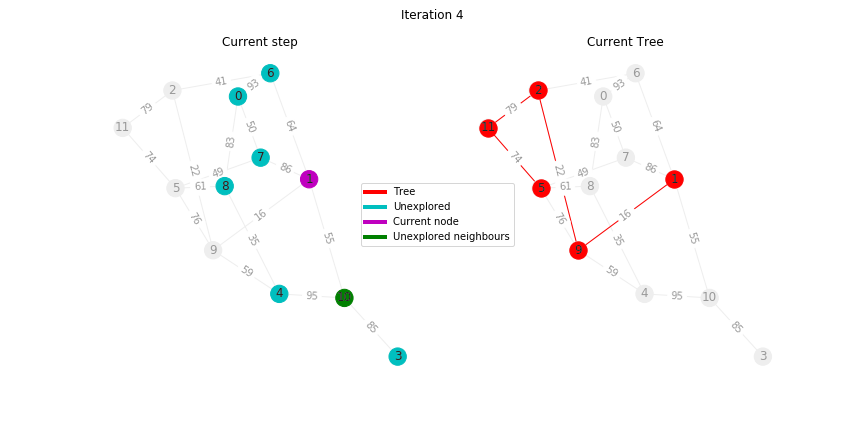
\includegraphics[width=\textwidth]{pricing/4.png}
    \end{subfigure}
    \caption{Algoritmo greedy per Vertex Cover}
\end{figure}
\subsection{Approccio con programmazione lineare}
\begin{multicols}{2}
\begin{definition}[Problema di PLI per vertex cover]
\begin{align*}
  \min \quad \sum_{i \in V} w_{i} x_{i}&\\  
  s.t. \quad x_{i}+x_{j} &\geq 1 \quad(i, j) \in E\\
  x_{i} &\in\{0,1\} \quad i \in V
\end{align*}
\end{definition}
\begin{lemma}[Massimale del peso di Vertex Cover come problema di PL]
    Sia \(S^*\) una vertex cover di peso minimo. Allora \(w_{LP} \leq w\rnd{S^*}\)
\end{lemma}
\begin{proof}[Massimale del peso di Vertex Cover come problema di PL]
    La \textbf{vertex cover} di \(G\) corrisponde alle soluzioni intere del problema di programmazione intera associato, pertanto il minimo di \(\min \left(w^{t} x : \overrightarrow{1} \geq x \geq 0, A x \geq 1\right)\) su tutti i vettori interi \(x\) corrisponde alla vertex cover di peso minimo. Per ottenere il minimo del problema di programmazione lineare, consentiamo ad \(x\) di assumere valori frazionari (rilassamento continuo), per cui il minimo del problema di programmazione lineare non risulta più grande di quello ottenuto tramite il problema di programmazione intera.
\end{proof}
\vfill\null
\columnbreak
\begin{lemma}[Massimale del peso di Vertex Cover come problema di PI]
    L'insieme \(S\) ottenuto tramite arrotondamento della soluzione di programmazione lineare è una \textbf{vertex cover} e \(w\rnd{S} \leq w_{\text{LP}}\)
\end{lemma}
\begin{proof}[Massimale del peso di Vertex Cover come problema di PI]
    Iniziamo provando che l'insieme \(S\) ottenuto arrotondando la soluzione di PL ottenuta sia una \textbf{vertex cover}. Consideriamo un lato \(e = \rnd{i,j}\): perché \(S\) sia una vertex cover almeno uno dei due vertici deve essere in \(S\). Una dei vincoli associati al problema di programmazione lineare intera risulta è \(x_{i}+x_{j} \geq 1\), per cui in ogni soluzione \(x^*\) che soddisfa questa disuguaglianza o \(x_{i}^{*} \geq \frac{1}{2}\) o \(x_{j}^{*} \geq \frac{1}{2}\). Pertanto almeno uno di questi due sarà arrotondato e o \(i\) o \(j\) sarà posto in \(S\).
    
    Consideriamo ora il peso \(w\rnd{S}\) di questa vertex cover. L'insieme \(S\) ha solo vertici con \(x_{i}^{*} \geq \frac{1}{2}\), per cui il problema di programmazione lineare \textbf{paga} almeno \(\frac{1}{2} w_{i}\) per il nodo \(i\) e paghiamo solo \(w_i\), al più pari al doppio.
    
    Più formalmente vale la seguente catena di disuguaglianze:
    \[w_{L P} w^{t} x^{*}=\sum_{i} w_{i} x_{i}^{*} \geq \sum_{i \in S} w_{i} x_{i}^{*} \geq \frac{1}{2} \sum_{i \in S} w_{i}=\frac{1}{2} w(S)\]
\end{proof}
\end{multicols}
\clearpage
\section{Pricing: problema dei passi separati}
\begin{problem}[Maximum Disjoint Paths Problem]
    Consideriamo un grafo direzionato \(G\), \(k\) coppie di nodi \(\left(s_{1}, t_{1}\right),\left(s_{2}, t_{2}\right), \ldots,\left(s_{k}, t_{k}\right)\) ed un intero \(c\) (capacità). Ogni coppia \(\rnd{s_j, t_j}\) vuole rappresentare una \textbf{richiesta di routing}, che richiede un cammino da \(s_j\) a \(t_j\). Una soluzione di questa istanza consiste in un sottoinsieme di richieste soddisfacibili e l'insieme dei cammini che le soddisfano tali che nessun lato viene percorso da due cammini distinti. 
    
    Il problema consiste nel soddisfare il maggior numero di richieste possibile. L'intero \(c\) rappresenta il massimo numero di lati condivisi che riterremo ammissibili: con \(c=1\) viene richiesto che i cammini siano completamente separati, con \(c>1\) consentiremo qualche sovrapposizione tra i cammini.
\end{problem}
\begin{definition}[Algoritmo greedy per Maximum Disjoint Paths Problem]
    Iniziamo da un insieme di richieste soddisfacibili vuoto e iteriamo finché non può essere identificato un nuovo cammino \(P_i\) senza sovrapposizioni. Consideriamo un tale cammino \(P_i\), il più corto possibile, che connette una coppia \(\rnd{s_j, t_j}\). Aggiungiamo il path \(P_i\) all'insieme della soluzione per connettere la richiesta identificata da \(\rnd{s_j, t_j}\).
\end{definition}
\begin{lemma}[Approssimazione dell'algoritmo greedy per Maximum Disjoint Paths Problem]
    L'algoritmo greedy per Maximum Disjoint Paths Problem è una \((2 \sqrt{m}+1)\)-approssimazione, dove \(m\) è il numero dei lati.
\end{lemma}
\begin{proof}[Approssimazione dell'algoritmo greedy per Maximum Disjoint Paths Problem]
    Consideriamo una soluzione ottima: sia \(I^*\) il suo insieme di coppie per cui il cammino è stato selezionato in questa soluzione ottima e sia \(P_i^*\) l'insieme dei cammini selezionati. Chiamiamo \(I\) l'insieme di coppie identificate dall'algoritmo greedy e sia \(P_i\) il cammino per ogni coppia identificata.
    
    La chiave della dimostrazione è fare una distinzione tra cammini lunghi e corti e considerarli separatamente. Chiameremo un cammino \textbf{lungo} se ha almeno \(\sqrt{m}\) lati, \textbf{corto} altrimenti. Sia \(I_S^*\) l'insieme degli indici in \(I^*\) corrispondenti a cammini corti. Il grafo \(G\) ha \(m\) lati, e ogni cammino lungo usa almeno \(\sqrt{m}\) lati, quindi possono esistere al più \(\sqrt{m}\) cammini lunghi in \(I^*\).
    
    Consideriamo ora i cammini corti in \(I^*\). Perché \(I^*\) contenga molte più richieste soddisfatte di \(I\) dovrebbero esserci tante coppie connesse in \(I^*\) che non sono connesse in \(I\). Consideriamo quindi coppie che sono connesse nella soluzione ottima utilizzando un cammino corto, ma che non vengono connesse dall'algoritmo greedy. Siccome il cammino \(P^*_i\) che connette \(s_i\) e \(t_i\) nella soluzione ottimale \(I^*\) è corto, la soluzione greedy lo avrebbe selezionato se fosse stato disponibile prima di selezionare un cammino più lungo, ma l'algoritmo greedy non lo ha connesso e quindi uno dei lati che compongono \(P^*_i\) deve essere in un altro cammino \(P_j\) selezionato precedentemente dall'algoritmo greedy. Diremo quindi che il lato \(e\) \textbf{blocca} il cammino \(P_i^*\).
    
    Ora la lunghezza dei cammini selezionati dall'algoritmo greedy aumenta monotamente, siccome ad ogni iterazione vengono scelti i cammini più corti. Il cammino \(P_j\) era selezionato prima considerando \(P^*_i\) e quindi deve essere più corto: \(\left|P_{j}\right| \leq\left|P_{i}^{*}\right| \leq \sqrt{m}\). Ne segue che anche \(P_j\) è \textbf{corto}. Siccome i cammini usati dalla soluzione ottima sono separati, ogni lato in un cammino \(P_j\) può \textbf{bloccare} al più un cammino \(P_i^*\). Ne segue che ogni cammino corto \(P_j\) blocca al più \(\sqrt{m}\) cammini nella soluzione ottima e quindi otteniamo la disequazione:
    \[
        \left|I_{s}^{*}-I\right| \leq \sum_{j \in I_{s}}\left|P_{j}\right| \leq\left|I_{s}\right| \sqrt{m}
    \]
    Consideriamo ora la soluzione ottima come composta da \(3\) tipi di cammini:
    \begin{enumerate}
        \item Cammini lunghi, di cui ne esistono al più \(\sqrt{m}\)
        \item Cammini che si trovano anche nella soluzione \(I\)
        \item Cammini corti che non si trovano anche in \(I\)
    \end{enumerate}
    Siccome \(\abs{I}\geq 1\) se almeno una richiesta risulta soddisfacibile, si può realizzare la disequazione:
    \[
        \left|I^{*}\right| \leq \sqrt{m}+|I|+\left|I_{s}^{*}-I\right| \leq \sqrt{m}+|I|+\sqrt{m}\left|I_{s}\right| \leq(2 \sqrt{m}+1)|I|
    \]
\end{proof}
\clearpage
\section{Problema del commesso viaggiatore (Christofides)}
\begin{multicols}{2}
\begin{problem}[Problema del commesso viaggiatore]
    Dato un insieme finito di vertici \(V\) e una funzione di distanza \(d: V^2 \rightarrow \R\) che soddisfa tutte le proprietà di una distanza (\textbf{non-negatività}, \textbf{simmetria} e \textbf{disuguaglianza triangolare}). L'obbiettivo è identificare il ciclo Hamiltoniano di lunghezza minima tra tutti i vertici.
\end{problem}
\begin{definition}[Christofides per TSP]
    Prima di tutto costruiamo un \textbf{albero ricoprente minimo} \(M\), quindi iniziando da un qualsiasi vertice percorriamo l'albero ricoprente \(M\) in senso anti-orario: questo percorso attraverso ogni lato una volta in ogni direzione, ma non è un \textbf{percorso Hamiltoniano} perché visita alcuni vertici più volte. 
    
    Possiamo eliminare i vertici già visitati come segue: iniziando da un punto arbitrario, percorriamo il ciclo realizzato ma marchiamo i vertici che incontriamo. Quando ne incontriamo uno visitato precedentemente lo saltiamo e passiamo direttamente al vertice successivo, iterando fino ad incontrare uno non visitato o il vertice iniziale. Il risultato è un \textbf{percorso Hamiltoniano}, e la sua lunghezza non è più grande del percorso originale grazie alla \textbf{disuguaglianza triangolare}.
    
    Sia ora \(O\) l'insieme dei vertici \textbf{ a grado dispari} di \(M\): questo insieme contiene tutte le foglie di \(M\) e potenzialmente anche qualche vertice interno. La cardinalità dell'insieme \(O\) è sicuramente pari perché la somma dei gradi di tutti i nodi deve essere pari essendo esattamente il doppio del numero di lati. Possiamo pertanto costruire un \textbf{matching perfetto} sul grafo completo che ha \(O\) come vertici e possiamo trovare un \textbf{matching minimo perfetto} \(P\) in tempo \textbf{polinomiale}.
    
    Consideriamo ora il grafo di lati \(E = E\rnd{P} \cup E\rnd{M}\): questo grafo potrebbe contenere archi multipli, dato che \(P\) ed \(M\) potrebbero sovrapporsi. Notiamo due aspetti importanti: tutti i nodi hanno grado \textbf{pari}, dato che aggiungiamo solo un lato di \(P\) incidente ad ogni nodo di \(O\) e vale che:
    \[
        d(E) \leq 3 d\left(T^{*}\right) / 2
    \]
    perché \(d(M) \leq d\left(T^{*}\right)\) e \(d(P) \leq d\left(T^{*}\right) / 2\). Siccome ogni nodo ha grado pari possiamo costruire un percorso Euleriano (cioè un ciclo che attraversa tutti gli archi esattamente una volta). Il percorso Euleriano è costruito iniziando da un vertice arbitrario e seguendo gli archi finché non si incontra il vertice iniziale nuovamente: se per caso fosse incontrato prima di finire il ciclo Euleriano basta continuare finché non si termina il percorso completamente. Il percorso Euleriano ottenuto ha lunghezza al più \( 3 d\left(T^{*}\right) / 2\). 
    
    Procediamo ora a comprimere il percorso a un ciclo Hamiltoniano saltando, come fatto precedentemente, i vertici già visitati e per disuguaglianza triangolare otteniamo un ciclo Hamiltoniano di lunghezza \( 3 d\left(T^{*}\right) / 2\).
\end{definition}
\begin{lemma}[\(1\degree\) approssimazione di Christofides]
    Il primo percorso Hamiltoniano identificato da Christofides (prima di ottenere il matching) è una \(2\)-approssimazione dell'ottimo.
\end{lemma}
\begin{proof}[\(1\degree\) approssimazione di Christofides]
    Sia \(T\) il ciclo risultante dalla prima approssimazione di Christofides per TSP, e sia \(T^*\) il ciclo ottimo. Sia \(e\) un lato qualsiasi del ciclo ottimo \(T^*\), quindi:
    \[
        d(T) \leq 2 d(M) \leq 2 d\left(T^{*}-e\right) \leq 2 d\left(T^{*}\right)
    \]
    La prima disuguaglianza deriva dal fatto che la lunghezza del ciclo iniziale ottenuto dall'\textbf{albero ricoprente minimo} \(M\), dato che ogni lato di \(M\) è attraversato esattamente due volte, e il ciclo ottenuto saltando alcuni vertici non è peggiore per la \textbf{disuguaglianza triangolare}. La seconda disuguaglianza deriva dal fatto che \(T^{*}-e\) è un albero ricoprente e quindi \(d(M) \leq d\left(T^{*}-e\right)\), dato che \(M\) è un albero ricoprente minimo. Infine la terza disuguaglianza deriva dal fatto che tutte le disuguaglianze sono non-negative. 
\end{proof}
\begin{lemma}[\(2\degree\) approssimazione di Christofides]
    Il secondo (e ultimo) percorso Hamiltoniano identificato da Christofides (prima di ottenere il matching) è una \(\frac{3}{2}\)-approssimazione dell'ottimo.
\end{lemma}
\begin{proof}[\(2\degree\) approssimazione di Christofides]
    Sia \(N^*\) il ciclo Hamiltoniano minimo costruito sull'insieme dei nodi a \textbf{grado dispari} \(O\) e siano \(N_1\) ed \(N_2\) i due \textbf{matching perfetti} su \(O\) ottenuti scegliendo alternando i lati di \(N^*\). Allora:
    \[
        d(P) \leq \min \rnd{d\left(N_{1}\right), d\left(N_{2}\right)} \leq d\left(N^{*}\right) / 2 \leq d\left(T^{*}\right) / 2
    \]
    La prima disuguaglianza si ottiene dal fatto che \(N_1\) ed \(N_2\) sono \textbf{matching perfetti} per \(O\) e \(P\) è un \textbf{matching minimo perfetto} su \(O\). La seconda disuguaglianza deriva dal fatto che il minimo di \(d\left(N_{1}\right)\) e \(d\left(N_{2}\right)\) è al più la media tra i due. Per la terza e ultima disuguaglianza, otteniamo il ciclo Hamiltoniano minimo (soluzione del TSP) su \(O\) dalla soluzione ottima \(T^*\) saltando i vertici pari. Per la \textbf{disuguaglianza triangolare}, la lunghezza del percorso ottenuto non è peggiore di \(d\rnd{T^*}\) e \(d\rnd{N^*}\) non è peggiore perché è un ciclo ottimo su \(O\).
    
    Consideriamo ora il grafo di lati \(E = E\rnd{P} \cup E\rnd{M}\). Vale che:
    \[
        d(E) \leq 3 d\left(T^{*}\right) / 2
    \]
    perché \(d(M) \leq d\left(T^{*}\right)\) e \(d(P) \leq d\left(T^{*}\right) / 2\) siccome costruiamo il ciclo Hamiltoniano selezionando un sottoinsieme degli archi di \(E\) risulta chiaramente che il ciclo ottenuto è una \(\frac{3}{2}\)-approssimazione del ciclo ottimo \(T^*\) 
\end{proof}
\end{multicols}
\end{document}